\documentclass[11pt,letterpaper]{article}

\usepackage{import}
\import{../../../../LaTeX}{basic}

\title{\textbf{Math 55a Problem Set 2}}

\begin{document}
\maketitle
\setcounter{page}{0}
\thispagestyle{empty}

\begin{itemize}
  \item How long did this assignment take you? -- about 14 hours
  \item How hard was it? -- some problems were trivial, others were pretty hard, overall tough
  \item What resources did you use and how much help did you need? - I collaborated with Yunseo Choi, Eliot Hodges, Gregory Li, Swati Goel, AJ LaMotta
  \item Did you have any prior experience with this material? -- Yes, I have a pretty solid group theory and abstract algebra background.
\end{itemize}

\pagebreak
\begin{problem}
  Describe a polygon in $\R^2$ whose symmetry group is $\Z /3$. What is the fewest number of vertices that such a polygon could have?
\end{problem}

Every plane symmetry is either a rotation (of order $\geq 2$) or a reflection (order $2$). Since $\Z /3$ only contains elements of order $3$, the shape must only have rotational symmetry by $\pm 2\pi /3$ and no reflectional symmetry. This implies that the shape must have $3n$ vertices, since every vertex must have two other corresponding vertices $2\pi /3$ and $4\pi /3$ radians further along the unit circle (the case when the vertex is at $(0,0)$ leads to a degenerate polygon so we won't consider it). It's fairly clear to see that no triangle can work, since the equilateral triangle has reflectional symmetry. We claim that a shape with $6$ vertices is minimal. Consider the ``offset star'' shown in the following figure:

\begin{center}
  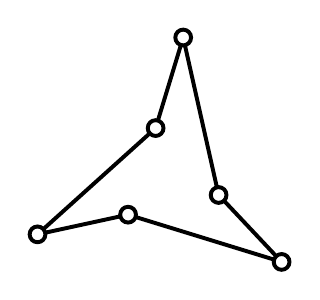
\begin{tikzpicture}[scale=0.5]
    \draw [line width=0.5mm, black] (-1.4,4.4) -- (-0.5,0.4) -- (1.1,-1.3) -- (-2.8,-0.1) -- (-5.1,-0.6) -- (-2.1, 2.1) -- cycle;
    \draw [fill=white, line width=0.5mm] (-1.4,4.4) circle (2mm) (-0.5,0.4) circle (2mm) (1.1,-1.3) circle (2mm) (-2.8,-0.1) circle (2mm) (-5.1,-0.6) circle (2mm) (-2.1, 2.1) circle (2mm);
  \end{tikzpicture}
\end{center}
This clearly exhibits a symmetry group of $\Z /3$, since it has no reflections and only rotations by $\pm 2\pi /3$. So $6$ is the smallest number of vertices such a shape can have.

\pagebreak
\begin{problem}
  Let $G$ be the set of {\em affine transformations} of the real line, i.e. maps $f_{a,b} : \R \to \R$ of the form $f_{a,b} : x \mapsto ax + b$ for some $a,b\in \R$ with $a\neq 0$.
  \begin{enumerate}
    \item Show that $G$ is a group, with group law given by composition.
    \item What is the center of $G$? (Recall the center of a group $G$ is the subgroup of elements which commute with all other elements, $Z(G)=\{a\in G : \forall x\in G, ax=xa\}$.)
    \item Show that the subsets $H=\{ f_{a,b} : a=1\}$ and $K=\{f_{a,b} : b=0\}$ are subgroups of $G$. Which one is normal, and what is the quotient of $G$ by that subgroup?  
  \end{enumerate}
\end{problem}

\textbf{(1)} Associativity follows because function composition is associative. The identity element is $f_{1,0}$. Lastly, the inverse of an element $f_{a,b}$ is $f_{1 /a, -b /a}$.

\textbf{(2)} We claim that the center is $\{ f_{1,0} \}$. To show this, suppose $f_{a,b}\in Z(G)$. Then $f_{a,b}f_{2,0}=f_{2,0}f_{a,b}$. So $a(2x)+b=2(ax+b)$, and so it follows that $b=2b$ so $b=0$. Next, we also have $f_{a,b}f_{0,1}=f_{0,1}f_{a,b}$. So $a(x+1)=ax+1$. This implies that $a-1=0$ so $a=1$. This shows that $f_{a,b}=f_{1,0}$, and so the center is trivial.

\textbf{(3)} To show that $H$ is a subgroup, observe that $f_{1,a}f_{1,b}=f_{1,a+b}$ and $f^{-1}_{1,a}=f_{1,-a}$. To show that $K$ is a subgroup, observe that $f_{a,0}f_{b,0}=f_{ab,0}$ and $f^{-1}_{a,0}=f_{1 /a, 0}$.    

We claim that the normal subgroup is $H$. Let $f_{a,b}\in G$. Then $f_{a,b}f_{1,c}=ax+ca+b=f_{1,ca}f_{a,b}$. So $f_{a,b}H=Hf_{a,b}$. 

Next we'll show that $G /H \cong (\R^*, \times)$. Consider the homomorphism $f : G \to (\R^*, \times)$ given by $f_{a,b} \mapsto a$. This map is surjective, and its kernel is $H$. So by the first isomorphism theorem, $G /H \cong (\R^*, \times)$.   

\pagebreak
\begin{problem}
  Let $G=S^1=\{ z\in \Z : |z|=1\}$ be the group of complex numbers of modulus $1$, with multiplication. Let $H\subset G$ be the subgroup $\{\pm 1\}$. Show that the quotient $G /H$ is isomorphic to $G$.   
\end{problem}

Consider the map $f : S^1\to S^1 : x \mapsto x^2$. This is clearly a group homomorphism, and is surjective because we can always find at least one square root of a modulus $1$ complex number. The kernel of this map is exactly the subgroup $H$, so by the first isomorphism theorem, we have an induced isomorphism $\widetilde{f} : S^1 /\{\pm 1\} \to S^1$.  

\pagebreak
\begin{problem}
  Let $G$ be the group of rotations preserving a cube in $\R^3$. Show that $G$ is isomorphic to the symmetric group $S_4$ (permutations of a four-element set).  
\end{problem}

We claim that each symmetry of a cube uniquely corresponds to a permutation of its $4$ diagonals. For example, the following labeling gives such an isomorphism:

\begin{center}
  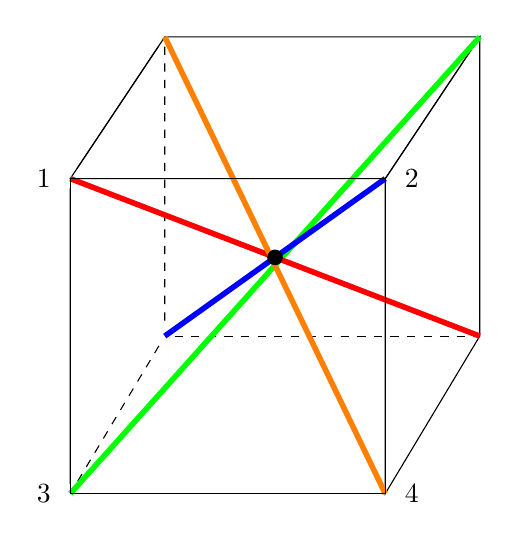
\begin{tikzpicture}
    \node[label={left:1}] (1) at (0.6, 4) {};
    \node[label={right:2}] (2) at (4.6, 4) {};
    \node[label={left:3}] (3) at (0.6, 0) {};
    \node[label={right:4}] (4) at (4.6, 0) {};
    \node (5) at (1.8, 5.8) {};
    \node (6) at (5.8, 5.8) {};
    \node (7) at (1.8, 2) {};
    \node (8) at (5.8, 2) {};
    
    \draw (1.center) -- (2.center) -- (6.center) -- (5.center) -- cycle;
    \draw (2.center) -- (4.center) -- (8.center) -- (6.center) -- cycle;
    \draw (3) -- (1) -- (5);
    \draw[dashed] (5) -- (7) -- (3);
    \draw[dashed] (7) -- (8);
    
    \draw[color=green, line width=2] (3.center) -- (6.center);
    \draw[color=red, line width=2] (1.center) -- (8.center);
    \draw[color=blue, line width=2] (2.center) -- (7.center);
    \draw[color=orange, line width=2] (4.center) -- (5.center);

    \draw (1.center) -- (2.center) -- (4.center) -- (3.center) -- cycle;

    \node[inner sep=2pt,circle,fill,color=black] (center) at (3.2, 3) {};
\end{tikzpicture}
\end{center}

It's pretty clear to see that every symmetry of a cube permutes the diagonals and that every permutation of the diagonals represents a symmetry of the cube. This shows that $G$ is isomorphic to $S_4$. This map must also be a homomorphism. Suppose the diagonals are labeled $1,2,3,4$ as in the diagram. Suppose $g,h$ are symmetries of the cube, each mapping the diagonal $i\mapsto g(i)$ and $i \mapsto h(i)$ respectively. Then $g\circ h$ maps the diagonal $i\mapsto g(h(i))$. So we have an isomorphism.        

\pagebreak
\begin{problem}
  Show that, if $G$ is a finite group and $H\subset G$ is a subgroup of index $2$ then $H$ is a normal subgroup of $G$. 
\end{problem}

We must show that $aH=Ha$ for all $a\in G$. If $a\in H$, we are done since $aH=Ha=H$. So suppose $a\notin H$. Then the (left) cosets $H$ and $aH$ are disjoint, and their union is $G$, since both have size $|G|/2$. Now consider the (right) coset $Ha$. Suppose $ha\in Ha$. Since $ha\in G$, either $ha\in H$ or $ha\in aH$. If $ha\in aH$ then we are done, but if $ha\in H$, then $h^{1}ha=a\in H$, a contradiction. So $ha\in aH$ and hence $aH = Ha$. This proves that $H$ is normal.                   

\pagebreak
\begin{problem}
  The dihedral group $D_n$ is the group of order $2n$ consisting of all symmetries (rotations and reflections) of the regular $n$-gon in the plane. Find all normal subgroups of $D_n$.
\end{problem}

For this problem, we'll use the following presentation of $D_n$:
\[ D_n = \big\langle r,s : \mathrm{ord}(r)=n, \mathrm{ord}(s)=2, sr^ks=r^{-k}\big\rangle\] 
We claim that for any $n$, the normal subgroups of $D_n$ are:
\begin{itemize}
  \item For any $d|n$, the subgroup $\big\langle r^d \big\rangle$. 
  \item If $n$ is even, the subgroups $\big\langle r^2, sr\big\rangle$ and $\big\langle r^2, s \big\rangle$. 
\end{itemize}

First we'll show that every normal subgroup of index $2$ must be either $\big\langle r \big\rangle$ or $\big\langle r^2, sr\big\rangle$ and $\big\langle r^2, s \big\rangle$ if $n$ is even. 
  
Suppose $N\subset D_n$ is a normal subgroup of index $2$. Then $D_n /N\cong \{\pm 1\}$ so there is a homomorphism $D_n \to \{\pm 1\}$. Conversely for every homomorphism $D_n \to \{\pm 1\}$ with nontrivial kernel, we get an index $2$ normal subgroup, namely the kernel. So to classify index $2$ subgroups of $D_n$ it suffices to look at $D_n \to \{\pm 1\}$. There are $4$ options for these maps, determined by where the generators map to. Suppose $f : D_n \to \{\pm 1\}$ is a homomorphism.
\begin{itemize}
  \item {\bf{\und{Case 1:}}} $f(r)=1, f(s)=1$. This case isn't interesting because $\ker f=D_n$.
  \item {\bf{\und{Case 2:}}} $f(r)=-1, f(s)=1$. In this case, $f(r^n)=f(r)^n=(-1)^n=1$ so $n$ must be even. The kernel of this map is exactly $\big\langle r^2, s \big\rangle$.
  \item {\bf{\und{Case 3:}}} $f(r)=1, f(s)=-1$. The kernel of this map is exactly $\big\langle r \big\rangle$.
  \item {\bf{\und{Case 4:}}} $f(r)=-1, f(s)=-1$. In this case we have $f(r^n)=f(r)^n=(-1)^n=1$ so $n$ must be even, and the kernel of this map is exactly $\big\langle r^2, s \big\rangle$.        
\end{itemize} 
Now suppose $N\subset D_n$ is an arbitrary normal subgroup of $D_n$. We'll show that it must be equivalent to a subgroup in the list. There are two cases:
\begin{itemize}
  \item {\bf\und{Case 1:}} $N$ contains no elements of the form $sr^k$. Then $N$ is a subgroup of $\big\langle r \big\rangle$ which is a cyclic group so $N$ must be cyclic, and hence of the form $\big\langle r^d \big\rangle$ for some $d|n$.  
  \item {\bf\und{Case 2:}} $sr^k \in N$ for some $k$. Then $sr^m(sr^k)r^{-m}s=sr^{2m-k}\in N$. 
  \begin{itemize}
    \item {\bf\und{Case 2a:}} If $n$ is odd, this implies that every $sr^m\in N$, and so by closure of the subgroup, $s\cdot sr^k=r^k$ implies that every $r^k\in N$ so $N=D_n$. 
    \item {\bf\und{Case 2b:}} If $n$ is even, this implies that either $\{s,sr^2,sr^4,\ldots\}\subset N$ or $\{sr,sr^3,\ldots\}\subset N$. In both cases, it also follows that $\{r^2,r^4,\ldots\}\subset N$. (Since $s\cdot sr^2=r^2$ in the former case and $sr\cdot sr^3=r^2$ in the former case). So assuming $N\neq D_n$, we have that $N=\big\langle r^2, sr\big\rangle$ or $N =\big\langle r^2, s \big\rangle$.    
  \end{itemize} 
\end{itemize}  
Since we've exhausted all possibilities for $N$, we are done.

\pagebreak
\begin{problem}
  Prove or provide a counterexample: If $A$ is a normal subgroup of $B$ and $B$ is a normal subgroup of $C$, then $A$ is a normal subgroup of $C$. 
\end{problem}

This is a false statement, observe the following counterexample:
\begin{counterexample}
  Let $C=D_4$, $B=\big\langle r^2, s\big\rangle$, and $A=\big\langle s\big\rangle$. $B$ is normal in $C$ by the previous problem, and $A$ is normal in $B$ because it is index $2$. However $A$ isn't normal in $C$. (as can be seen by the previous problem)     
\end{counterexample}

\pagebreak
\begin{problem}
  Find the order of the group $\GL_2(\Z /2)$ of $2\times 2$ matrices with entries in $\Z /2$ and nonzero determinant $(\mod 2)$. Is $\GL_2(\Z /2)$ isomorphic to another group we've encountered?
\end{problem}

We claim that $\GL_2(\Z /2)\cong S_3$, which would show that $|\GL_2(\Z /2)|=6$. Consider the map
\[ \varphi : \GL_2(\Z /2) \to \textrm{Perm}\left(\begin{bmatrix}0\\1\end{bmatrix}, \begin{bmatrix}1\\0\end{bmatrix}, \begin{bmatrix}1\\1\end{bmatrix}\right)\cong S_3\]
where each matrix $M\in \GL_2(\Z /2)$ is sent to the permutation given by $\bar{v} \mapsto M\bar{v}$. This is indeed a permutation since $M$ has determinant $1$ and hence is invertible. $\varphi$ also must be injective, since the action of a matrix on the unit vectors determines the matrix uniquely. Lastly, we'll show surjectivity. Suppose $f$.is a permutation. Then $\varphi^{-1}(f)$ is the matrix representing the linear transformation taking $e_1 \mapsto f(e_1)$ and $e_2 \mapsto f(e_2)$, where $e_1,e_2$ are the standard unit vectors.

So $\varphi : \GL_2(\Z /2) \to S_3$ is a bijection, and we can write out this map explicitly:
\begin{align*}
  &\begin{bmatrix}
    1&0\\0&1
  \end{bmatrix}\mapsto e 
  &\begin{bmatrix}
    1&0\\1&1
  \end{bmatrix}\mapsto (23)&\\
  &\begin{bmatrix}
    0&1\\1&0
  \end{bmatrix}\mapsto (12)
  &\begin{bmatrix}
    1&1\\1&0
  \end{bmatrix}\mapsto (123)&\\
  &\begin{bmatrix}
    1&1\\0&1
  \end{bmatrix}\mapsto (13)  
  &\begin{bmatrix}
    0&1\\1&1
  \end{bmatrix}\mapsto (132)&\\
\end{align*}

\pagebreak
\begin{problem}
  \begin{enumerate}
    \item Let $p$ be a prime number, and suppose $H\subset S_p$ is a subgroup of the group of permutations of $\{1,2,\dots,p\}$. Show that if $H$ contains the $p$-cycle $(123\dots p)$ and a transposition (a permutation that exchanges two elements and fixes all others), then $H=S_p$. (In other words: $S_p$ is generated by $(123\dots p)$ and by {\em any} transposition).
    \item Show that the conclusion of the first part may be false if we don't assume $p$ is prime (even though it is still true that $S_p$ is generated by $(123\dots p)$ and a {\em suitably chosen} transposition).
  \end{enumerate}
\end{problem}

\textbf{(1)} We'll actually prove a more general statement. Before stating it, let's prove a lemma.

\begin{lemma}
  Let $n\geq 2$ be any integer. Then $S_n$ is generated by $(123\cdots n)$ and $(12)$.  
\end{lemma}
\begin{proof}
Since $S_n$ is generated by transpositions, it suffices to show that any transposition $(a\quad b)$ can be expressed in terms of $(123\cdots n)$ and $(12)$. Note that
\[
  (a\quad a+1)=(123\cdots n)^a(12)(123\cdots n)^{-a}
.\] 
So we can generate all ``adjacent'' transpositions. For a general transposition $(a\quad b)$, we can write it as
\[
  (a\quad b)=(a\quad a+1)(a+1\quad b)(a\quad a+1)
.\]
By induction, we can keep writing $(a+1\quad b)$ in this form until we get down to an adjacent transposition, completing the proof.    
\end{proof}

To show that we can generate $(12)$ from $(123\cdots n)$ and an arbitrary transposition $(a\quad b)$, we'll actually prove a more general result.

\begin{proposition}
  Let $p\geq 2$ be a prime. Then $S_p$ is generated by any $p$-cycle $(a_1 a_2\cdots a_{p-1} a_p)$ and transposition $(a_i a_j)$.    
\end{proposition}
\begin{proof}
  First, we'll relabel $S_p$ so that $a_i=1$ and we'll rotate the $p$-cycle, so we now have $(1\cdots a_{p-1}a_{p}a_1 a_2\cdots )$ and $(1\quad a_j)$. Since $p$ is prime and $(1\cdots a_{p-1}a_{p}a_1 a_2\cdots )$ is a $p$-cycle, there must exist some $1\leq k \leq p-1$ such that $(1\cdots a_{p-1}a_{p}a_1 a_2\cdots )^k=(1 \quad a_j \cdots)$ is also a $p$-cycle. Relabeling $S_p$ again so that $a_j=2$ and so the other elements in the $p$-cycle line up accordingly, we have $(123\cdots p)$ and $(12)$. Since $(12)$ and $(123\cdots p)$ are generated, by the previous lemma we can generate all of $S_p$.        
\end{proof}

\textbf{(2)} In general, $(1\quad 1+k)$ and $(123\cdots n)$ will not generate $n$ provided that $(n,k)>1$. For instance, consider $(13)$ and $(1234)$ in $S_4$, and let $g\in G= \big\langle (13), (1234)\big\rangle$. Then $g(1)\equiv g(3)\mod 2$ because $(13)1\equiv (13)3\mod 2$ and $(1234)1\equiv (1234)3\mod 2$. (Likewise with $(1234)^{-1}$). This means that $(12)\notin G$ since $(12)1\not\equiv (12)3\mod 2$. So $G\neq S_n$.                 

\pagebreak
\begin{problem}
  Let $G$ be a finitely generated group, and $H \subset G$ a subgroup of finite index. Show that $H$ is finitely generated.
\end{problem}

\textit{(Hint: Choose a finite subset $S\subset G$ containing one representative of each coset of $H$, so every element of $G$ is the product of an element of $S$ and an element of $H$. Given a word in the generators of $G$ and their inverses, how do you rewrite it as the product of an element of $S$ and an element of $H$?)}
 
Since $H$ is a subgroup of finite index, say $[G : H]=m$, we have the partitioning
\[G=\bigsqcup_{i=1}^m s_iH\]
for some finite set of coset representatives $s_i\in G$. WLOG assume that $s_1=e$. Let $S=\{ s_1,s_2,\ldots, s_m\}$. Thus every $g\in G$ can be expressed as $g=sh$ for some $s\in S$ and $h\in H$. Consider the functions (not necessarily homomorphisms) $\beta : G \to H$ and $\alpha : G \to S$ defined in the natural way so that $g=\alpha(g)\beta(g)$ for all $g\in G$. 

Now let $\{ g_1,g_2,\ldots, g_n\}$ be the generating set for $G$, as well as inverses of the generators. (So that every $g\in G$ can be expressed as a word in $g_i$) We claim that the set $B=\{\beta(g_is_j)\}$ (where $i,j$ can range freely within their bounds) is a generating set for $H$.

\begin{proposition}
  Suppose $g_{p_1}g_{p_{2}}\cdots g_{p_k}=g\in G$ for some $p_i$ and $k>0$. Then $g=sb_1b_2\cdots b_k$ for some $s\in S$ and $b_i\in B$.    
\end{proposition}     
\begin{proof}
  We'll prove the claim by induction on $k$. For the base case of $k=1$ note that $g=g_{p_1}$ implies $g=\alpha(g_{p_1})\beta(g_{p_1})$. Here $\alpha(g_{p_1})\in S$ and $\beta(g_{p_1})\in B$ by definition. Now suppose the claim is true for $k$, and we are given an $g=g_{p_1}g_{p_{2}}\cdots g_{p_k}g_{p_{k+1}}$. Write $g_{p_{2}}\cdots g_{p_k}g_{p_{k+1}}=sb_2b_3\cdots b_kb_{k+1}$ by the inductive hypothesis. Then,
  \begin{align*}
    g_{p_{1}}g_{p_{2}}\cdots g_{p_k}g_{p_{k+1}}&=g_{p_1}sb_2b_3\cdots b_kb_{k+1}\\
    &=\alpha(g_{p_1}s)\beta(g_{p_1}s)b_2b_3\cdots b_kb_{k+1}\\
  \end{align*}
  Since $\alpha(g_{p_1}s)\in S$ and $\beta(g_{p_1}s)\in B$ we are done.       
\end{proof}

Now we'll show that $B$ generates $H$. By the above proposition, every $h\in H$ can be expressed as $h=sb_1 b_2 \cdots b_k$. However since $b_i\in H$, it follows that $s=hb_k^{-1}\cdots b_2^{-1}b_1^{-1}\in H$. So $s=e$ by the earlier WLOG assumption, and so $h=b_1b_2\cdots b_k$. This completes the proof, since $B$ is a finite generating set for $H$.      

\pagebreak
\begin{problem}
  Let $G$ be a non-abelian finite group, and consider its center $Z(G)=\{ a\in G : \forall x\in G, ax=xa \}$.
  \begin{enumerate}
    \item Show that $G /Z(G)$ is not a cyclic group.
    \item Show that at most $5 /8 ^\textrm{ths}$ of the pairs of elements of $G$ commute, i.e. the set $\{(a,b)\in G\times G : $  $|C|\leq\frac{5}{8}|G|^2$.
    \item Show that this bound is optimal, i.e. there is a group $G$ such that $|C|=\frac{5}{8}|G|^2$. 
  \end{enumerate} 
\end{problem}

\textbf{(1)} Suppose for the sake of contradiction that $G/ Z(G)$ was cyclic, say $G /Z(G)=\big\langle aZ(G)\big\rangle$. Then,
\[G=\bigsqcup_{i=0}^n a^iZ(G).\]
This means that every $g$ can be expressed as $g=a^iz$ for some $z\in Z(G)$. So for any two elements $g,h\in G$ with $g=a^iz_1$, $h=a^jz_2$. So $ghg^{-1}=a^iz_1(a^jz_2)z_1^{-1}a^{-i}=a^ia^ja^{-i}z_1z_2z_1^{-1}=a^jz_2=h$. So $g\in Z(G)$, which is a contradiction because this would imply that $G$ was abelian.          

\textbf{(2)} First note that since $G /Z(G)$ isn't cyclic, we have the bound $|Z(G)|\leq \frac{1}{4}|G|$, since the smallest non-cyclic group is of order $4$. 

Now for any $g\in G$, define $S(g)=\{x\in G : xgx^{-1}=g\}$. This is a subgroup of $G$, since if $x,y\in S(g)$, $xygy^{-1}x^{-1}=xgx^{-1}=g$ so $xy\in S(g)$. Likewise $e\in S(g)$ and $x^{-1}\in S(g)$. By Lagrange's theorem, $|S(g)|$ divides $|G|$. So if $g\in Z(G)$, then $S(g)=G$ and if $g\notin Z(G)$, then $|S(g)|\leq \frac{1}{2}|G|$. Putting this all together,
\begin{align*}
  |C|=\sum_{g\in G}|S(g)|&=\sum_{g\in Z(G)}|S(g)|+\sum_{g\notin Z(G)}|S(g)|\\&\leq |G|\cdot |Z(G)|+(|G|-|Z(G)|)\cdot \frac{1}{2}|G|\\
&\leq \frac{1}{4}|G|^2+\frac{3}{4}|G|\cdot \frac{1}{2}|G|\\
&=\frac{5}{8}|G|^2\end{align*}   

\textbf{(3)} We claim that $D_4$ satisfies this bound. Using the same presentation as in the proof of problem $6$, we'll calculate $|S(g)|$ for all $g\in D_4$. Using the list of subgroups of $D_4$ from PSET $1$ and some computation, we get:
\begin{center}
  \def\arraystretch{1.5}
  \begin{tabular}{ |c|c|c||c|c|c| }
    \hline
    $g\in D_4$ & $S(g)$ & $|S(g)|$ & $g\in D_4$ & $S(g)$ & $|S(g)|$ \\
    \hline
    \hline
    $e$ & $D_4$ & $8$ & $s$ & $\big\langle s, r^2 \big\rangle$ & $4$ \\  
    \hline
    $r$ & $\big\langle r \big\rangle$ & $4$ & $sr$ & $\big\langle sr, r^2 \big\rangle$ & $4$ \\ 
    \hline
    $r^2$ & $D_4$ & $8$ & $sr^2$ & $\big\langle s, r^2 \big\rangle$ & $4$  \\ 
    \hline
    $r^3$ & $\big\langle r \big\rangle$ & $4$ & $sr^3$ & $\big\langle sr, r^2 \big\rangle$ & $4$ \\
    \hline  
  \end{tabular}
\end{center}
Adding everything up, we get that $|C|=2\cdot 8+6\cdot 4=16+24=40=\frac{5}{8}\cdot 16^2$. 
\pagebreak
\begin{problem}
    Given a set $S$, let $\mathcal{E}\subset \mathcal{P}(S)$ be such that:
    \begin{enumerate}
        \item $S\in \mathcal{E}$.
        \item If $A\in \mathcal{E}$ then $S-A\in \mathcal{E}$.
        \item If $A,B\in \mathcal{E}$ then $A\cup B\in \mathcal{E}$ and $A\cap B\in \mathcal{E}$.
    \end{enumerate}

    Prove that if $S$ is finite then there is a set $T$ and a surjective map $f:S\to T$ such that $\mathcal{E}=\{f^{-1}(A),\ A\subset T\}$. What happens if $S$ is infinite?
\end{problem}

For the sake of clarity, we will refer to the pair $(S, \mathcal{E})$ satisfying conditions (1), (2), and (3) of the problem as a ``pseudo-measurable space'' and refer to $\mathcal{E}$ as a  ``pseudo-$\sigma$-algebra''. (In a real $\sigma$-algebra, countable unions and intersections as opposed to finite unions and intersections here)

\begin{lemma}\label{restrlemma}
    Suppose $(X, \sigma)$ is a pseudo-measurable space and suppose $Y\in\sigma$. Then $(Y, \restr{\sigma}{Y})$ is a pseudo-measurable space, where $\restr{\sigma}{Y} := \{ A\cap Y : A\in \sigma\}$.
\end{lemma}
\begin{proof}
    We can check all the conditions to show $\sigma\cap \mathcal{P}(Y)$ is a pseudo-$\sigma$-algebra.
    \begin{enumerate}
        \item It's clear that $Y\in \restr{\sigma}{Y}$.
        \item Suppose $A\in \restr{\sigma}{Y}$. Then $S-A\in \sigma$, so $(S-A)\cap Y = Y-A\in \restr{\sigma}{Y}$.
        \item Suppose $A,B \in \restr{\sigma}{Y}$. Then $A\cup B, A\cap B\in \sigma$. Since $A,B\subset Y$, it follows that $Y\cap (A\cup B) = A\cup B$ and $Y \cap (A\cap B) = A\cap B$ so $A\cup B, A\cap B\in \restr{\sigma}{Y}$.
    \end{enumerate}
    This proves that $\left(Y, \restr{\sigma}{Y}\right)$ is a pseudo-measurable space. 
\end{proof}

We can then rephrase the above problem somewhat:

\begin{lemma}
    Prove that for any finite set $S$ and pseudo-$\sigma$-algebra $\mathcal{E}$ on $S$, there exists a surjective function $f : S \to T$ such that $\mathcal{E}=f^{-1}(\mathcal{P}(T))$. (This last part is a slight abuse of notation.)
\end{lemma}

\begin{proof}
    We'll prove the claim by strong induction on the size of $S$.

    \begin{itemize}
        \item If $|S|=1$, the only possible pseudo-$\sigma$-algebra on $S$ is $\mathcal{E}=\{\varnothing, S\}$, so we can let $f : S \to \{0\}$.
        \item Now suppose the claim is true for all sets of size less than $N$. Now let $|S|=N$. We can assume WLOG that $\mathcal{E}$ contains a proper subset of $S$, say $A\in\mathcal{E}$. (Otherwise, $\mathcal{E}=\{\varnothing, S\}$ and we'd be done.) Consider the following two pairs:
        \[\left(S-A, \restr{\mathcal{E}}{S-A}\right)\textrm{ and }\left(A, \restr{\mathcal{E}   }{A}\right)\]
        By Lemma~\ref{restrlemma}, these are both pseudo-measurable spaces, and $|S-A|<N$ and $|A|<N$ since $A$ was assumed to be a proper subset of $S$. Hence, by the inductive hypothesis, there exist functions
        \[ f_1 : \left(S-A, \restr{\mathcal{E}}{S-A}\right) \to T_1\textrm{ and } f_2 : \left(A, \restr{\mathcal{E}}{A}\right) \to T_2 \]
        satisfying $\restr{\mathcal{E}}{S-A} = f_1^{-1}(\mathcal{P}(T_1))$ and $\restr{\mathcal{E}}{A} = f_2^{-1}(\mathcal{P}(T_2))$. We can then construct a function,
        \[ f : S = (S-A)\sqcup A \to T_1\sqcup T_2 = T\]
        defined in the obvious way. We can show that this function satisfies $\mathcal{E} = f^{-1}(\mathcal{P}(T))$, which would complete the induction.
        \begin{itemize}
            \item First, suppose $B\in f^{-1}(\mathcal{P}(T))$, say $B=f^{-1}(H)$, where $H\subset T$. Then $H=H_1\sqcup H_2$ where $H_1\subset T_1$ and $H_2\subset T_2$. By the definition of $f$, it follows that $f^{-1}(H)=f_1^{-1}(H_1)\sqcup f_2^{-1}(H_2)$. Since $f^{-1}_1(H_1)\in \restr{\mathcal{E}}{S-A}$ and $f^{-1}_2(H_2)\in \restr{\mathcal{E}}{A}$, (by definition of $f_1$ and $f_2$), it follows that $B = f_1^{-1}(H_1)\sqcup f_2^{-1}(H_2) = (S-A)\cap E_1 \cup A\cap E_2$ for some $E_1, E_2\in \mathcal{E}$. Since this expression only contains complements, unions, and intersections, it must be in the pseudo-$\sigma$-algebra, so $B\in \mathcal{E}$.
            \item Conversely, suppose $B\in \mathcal{E}$. $B$ can be decomposed as $B=B_1\sqcup B_2$ where $B_1=(S-A)\cap B$ and $B_2=A\cap B$. Then $B_1\in \restr{\mathcal{E}}{S-A}$ and $B_2\in \restr{\mathcal{E}}{A}$ so $B_1\in f_1^{-1}(\mathcal{P}(T_1))$ and $B_2\in f_2^{-1}(\mathcal{P}(T_2))$. By a similar argument to the first part, we can conclude that $B\in f^{-1}(\mathcal{P}(T))$.
        \end{itemize}

        Now since $\mathcal{E} \subset f^{-1}(\mathcal{P}(T))$ and $f^{-1}(\mathcal{P}(T)) \subset \mathcal{E}$, it follows that $\mathcal{E} = f^{-1}(\mathcal{P}(T))$, so the claim follows by induction. \qedhere
    \end{itemize}
\end{proof}

The case when $S$ is infinite is not as simple. However if $\mathcal{E}$ is finite, then we can modify the induction to be on the size of $\mathcal{E}$ and get the same result. In general however, the claim is not true. 

\begin{counterexample}
    Let $\{p_i\}_{i\geq 0}$ be the set of all prime integers. Consider the pseudo-measurable space $(\N, \mathcal{E})$ where $\mathcal{E} = \langle \{p_i\}_{i\geq 0}\rangle$ is the pseudo-$\sigma$-algebra generated by $\{p_i\}_{i\geq 0}$. Then there does not exist a set $T$ and surjective map $f : \N \to T$ such that $\mathcal{E} = f^{-1}(\mathcal{P}(T))$.   
\end{counterexample}
\begin{cproof}
    Suppose for the sake of contradiction that there did exist some map $f : \N \to T$ satisfying the conditions of the claim. Since $f$ is surjective, and $\mathcal{E}=f^{-1}(\mathcal{P}(T))$, $T$ must be countably infinite so we can assume WLOG that $T=\N$. Consider the set $A=\{p_i\}_{i\geq 0}$. By assumption, $A\in \mathcal{E}$ since $A=f^{-1}\left(\{f(p_i)\}_{i\geq 0}\right)$. This is a contradiction, because $A$ cannot be expressed as a finite combination of complemenets, intersections, and unions of $\{p_i\}$.
\end{cproof}

So generally, it appears the claim holds true for finite pseudo-$\sigma$-algebras but in general does not hold true for infinite pseudo-$\sigma$-algebras.

\end{document}